\documentclass{article}
\usepackage[utf8]{inputenc}
\usepackage{amsmath}
\usepackage{amssymb}
\usepackage{amsfonts}
\usepackage{graphicx}
\usepackage{tikz}
\usetikzlibrary{angles,fit,arrows.meta,calc,math,matrix,intersections,through,backgrounds,cd}
\usepackage{pgfplots}
\pgfplotsset{compat=1.18}
\usepackage{geometry}
\geometry{a4paper, margin=1in}
\usepackage{booktabs} % For professional looking tables

\title{Visualization and Analysis of $4_1$ Knot Paths in (U,V) Space and $e^V$ Weighted Area}
\author{Manus}
\date{\today}

\begin{document}
\maketitle

\section{Introduction}
This document explores the second research direction: the visualization and preliminary analysis of geometric properties of paths associated with the figure-eight knot ($4_1$) within the $(U,V)$ reference space. A key focus is understanding the $e^V$ weighted area, which arises in the geometric interpretation of global arithmetic torsion, $\mathcal{T}(S) = \iint_{\Sigma_S} e^V dV \wedge dU$.

The $4_1$ knot (Figure-Eight Knot) is the simplest hyperbolic knot and serves as a fundamental example for exploring connections between knot theory and Arithmetic Expression Geometry (AEG).

\begin{figure}[h!]
    \centering
    \documentclass{standalone}
\usepackage{amsthm}
\usepackage{amssymb}
\usepackage{amsfonts}
\usepackage{amsmath}
\usepackage{mathtools}

\usepackage{pgf}
\usepgflibrary{fpu}
\usepackage{pgfplots}
\usepackage{tikz}
\usetikzlibrary{angles,fit,arrows,calc,math,matrix,intersections,through,backgrounds,cd}
\usepackage{tkz-euclide}
\usepackage{tkz-graph}
\usepackage{graphicx}
\pgfplotsset{compat=1.18}

\begin{document}

        \tikzmath{
                \one = 1;
                \base = 2.618033988749;
                \offset = 15.8888888;
                \valofpi = 3.1415926;
                \anglei = 3.1415926;
                \angleo = 3.1415926;
        }

        \begin{tikzpicture}[scale=1.0]
                % 1. 绘制坐标轴
                \draw[black, line width=0.6pt, ->]
                (\offset,0) to[out=90,in=270] (\offset,15.5)
                node [anchor=south] {y};

                \draw[black, line width=0.6pt, ->]
                (-7.5,0) to[out=0,in=180] (18,0)
                node [anchor=west] {x};

                % 2. 绘制 x 和 y 坐标轴刻度
                \foreach \x in {-25,...,2} {
                        \node [anchor=north] at (\x/9*8 + \offset, 0) {\x};
                }
                \foreach \y in {1,...,17} {
                        \node [anchor=-135] at (18, \y/9*8) {\y};
                }

                % 3. 浅灰色水平网格线
                \foreach \t in {17,...,1} {
                        \draw [lightgray, line width=0.6pt]
                        (-7.5,\t/9*8)
                        to[out=0,in=180]
                        (18,\t/9*8);
                }

                % 4. 浅灰色竖直网格线
                \foreach \t in {-26,...,2} {
                        \draw [lightgray, line width=0.6pt]
                        (\t/9*8 + \offset, 0)
                        to[out=90,in=270]
                        (\t/9*8 + \offset, 15.5);
                }




        \end{tikzpicture}
\end{document}
 % Assumes knot_4_1.tex is in figures subdirectory
    \caption{The Figure-Eight Knot ($4_1$).}
    \label{fig:knot_4_1_q2}
\end{figure}

\section{Geometric Interpretation of Arithmetic Torsion}
Material 5 of the provided research background introduces a geometric interpretation of the global arithmetic torsion for a path $S$ (typically a relator in the knot group $G(K)$) as an integral over a surface $\Sigma_S$ in a $(U,V)$ reference space:
\[
\mathcal{T}(S) = \iint_{\Sigma_S} e^V dV \wedge dU
\]
Here, $U$ and $V$ are coordinates in a 2-dimensional space where arithmetic operations of addition and multiplication are represented as translations. For an arithmetic expression $P$, $U(P)$ can be thought of as related to the additive structure and $V(P)$ to the multiplicative structure. Specifically, if an expression involves $m$ multiplications by a factor $t_k$ at each step, $V$ can accumulate as $V = \sum \ln t_k$. If $t$ is a constant parameter for $m$ multiplicative operations, $V = m \ln t$.

\section{Visualizing Paths in (U,V) Space}

\subsection{Conceptual Path Representation}
As described in the user's documentation (e.g., `knots_01.tex`), paths corresponding to relators of $G(4_1)$ can be visualized in the $(U,V)$ plane. The path traces a trajectory based on arithmetic operations, and a closed loop (formed by $S$ and potentially $S_{\text{rev}}$ or other segments) encloses the region $\Sigma_S$.

\begin{figure}[h!]
    \centering
    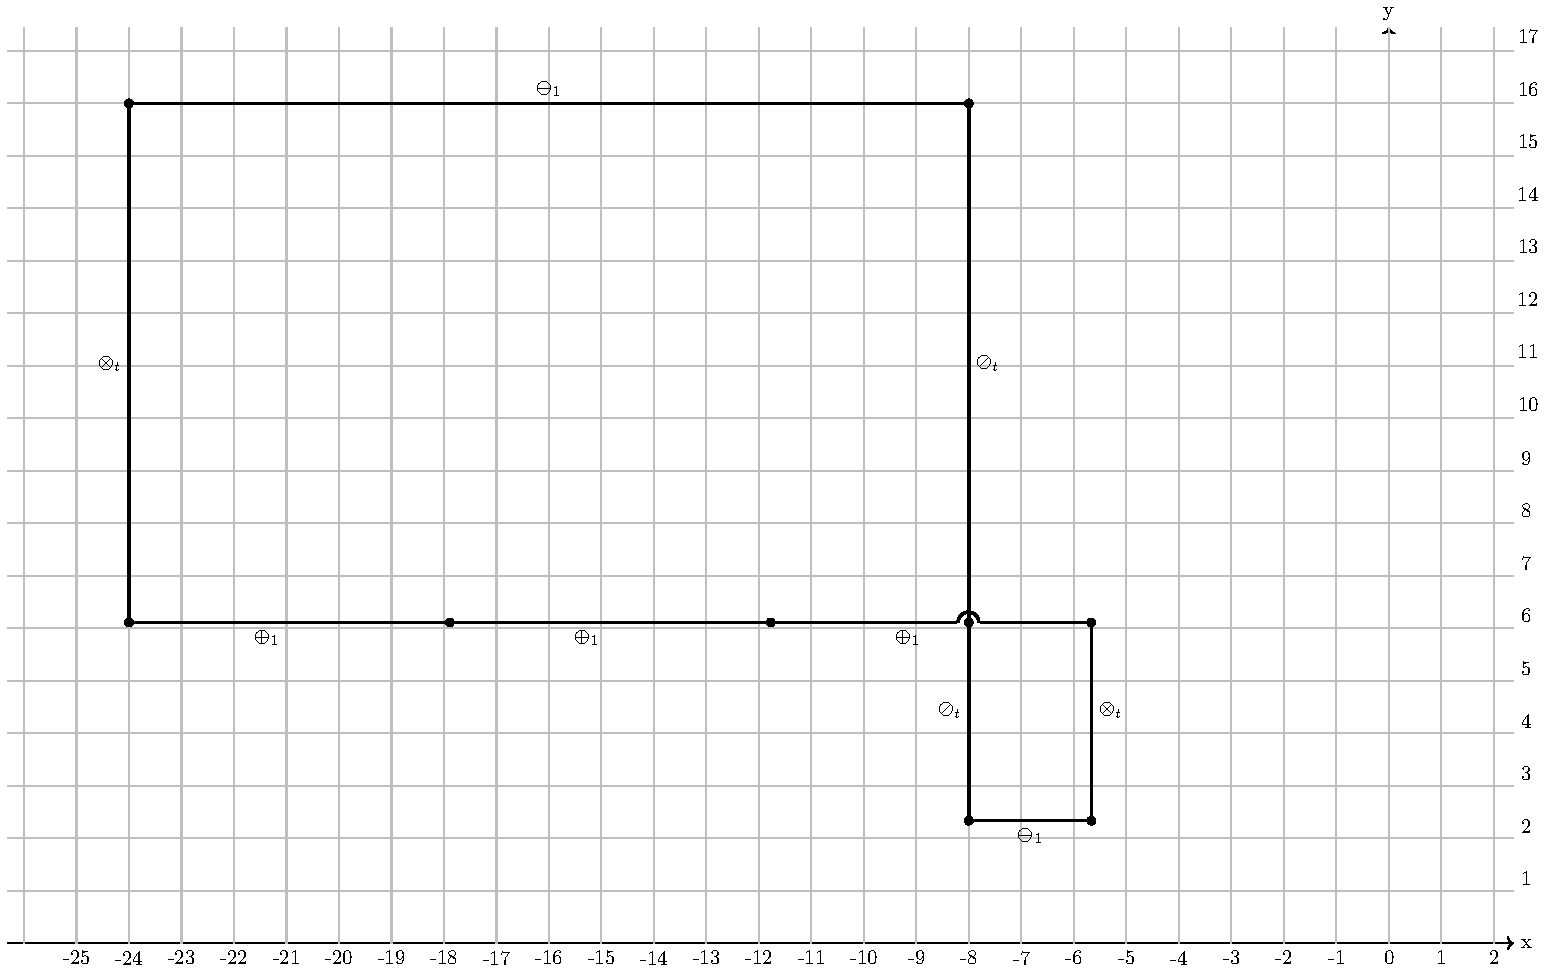
\includegraphics[width=0.7\textwidth]{../../images/knot_4_1.pdf} % User's preferred schematic
    \caption{Schematic representation of a relator path in the (U,V) arithmetic expression space (conceptual, from repository).}
    \label{fig:uv_path_conceptual_q2}
\end{figure}

Figure \ref{fig:uv_path_conceptual_q2} shows the user's conceptual schematic for such a path.

\subsection{Worked Example: Path Construction for $S = \text{aBAABabb}$ with $t=2$}
To make the concept concrete, let us consider the specific path $S = \text{aBAABabb}$ and map its operations to movements in the $(U,V)$ plane. Following user feedback and common context in AEG discussions, we will use $t=2$. The mapping is:
\begin{itemize}
    \item Operation `a` (multiplication by $t=2$) corresponds to a change $(0, \ln 2)$ in $(U,V)$.
    \item Operation `A` (multiplication by $t^{-1}=1/2$) corresponds to a change $(0, -\ln 2)$ in $(U,V)$.
    \item Operation `b` (addition of $1$) corresponds to a change $(1, 0)$ in $(U,V)$.
    \item Operation `B` (addition of $-1$) corresponds to a change $(-1, 0)$ in $(U,V)$.
\end{itemize}

Starting at $(U_0, V_0) = (0,0)$:
\begin{enumerate}
    \item $P_0 = (0,0)$
    \item `a`: $(U_1, V_1) = (0,0) + (0, \ln 2) = (0, \ln 2)$
    \item `B`: $(U_2, V_2) = (0, \ln 2) + (-1,0) = (-1, \ln 2)$
    \item `A`: $(U_3, V_3) = (-1, \ln 2) + (0, -\ln 2) = (-1, 0)$
    \item `A`: $(U_4, V_4) = (-1, 0) + (0, -\ln 2) = (-1, -\ln 2)$
    \item `B`: $(U_5, V_5) = (-1, -\ln 2) + (-1,0) = (-2, -\ln 2)$
    \item `a`: $(U_6, V_6) = (-2, -\ln 2) + (0, \ln 2) = (-2, 0)$
    \item `b`: $(U_7, V_7) = (-2, 0) + (1,0) = (-1, 0)$ (This point is $P_3$)
    \item `b`: $(U_8, V_8) = (-1, 0) + (1,0) = (0, 0)$ (This point is $P_0$, the path closes)
\end{enumerate}

This path $S = \text{aBAABabb}$ forms a closed loop in the $(U,V)$ plane. The surface $\Sigma_S$ is the region enclosed by this path.

\begin{figure}[h!]
    \centering
    \resizebox{0.9\textwidth}{!}{\documentclass{standalone}
\usepackage{tikz}
\usetikzlibrary{arrows.meta} % For nicer arrowheads

\begin{document}
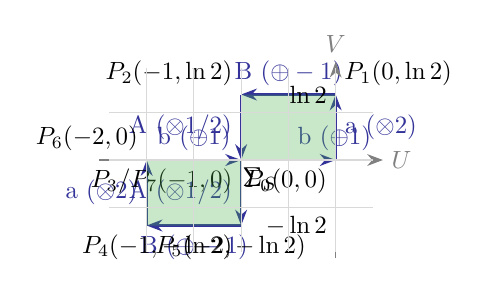
\begin{tikzpicture}[scale=1.2, every node/.style={scale=0.9, auto}]
    % Define coordinates for the path aBAABabb with t=2 (ln t = ln 2)
    \pgfmathsetmacro{\lnTwo}{ln(2)} % Define ln(2) for V coordinates

    \coordinate (P0) at (0,0);            % Start
    \coordinate (P1) at (0,\lnTwo);       % after a
    \coordinate (P2) at (-1,\lnTwo);      % after B
    \coordinate (P3) at (-1,0);           % after A
    \coordinate (P4) at (-1,-\lnTwo);     % after A
    \coordinate (P5) at (-2,-\lnTwo);     % after B
    \coordinate (P6) at (-2,0);           % after a
    \coordinate (P7) at (-1,0);           % after b (Note: P7 is same as P3)
    \coordinate (P8) at (0,0);            % after b (Note: P8 is same as P0, path closes)

    % Draw path segments with labels for operations
    \definecolor{pathcolor}{rgb}{0.2,0.2,0.6}
    \draw[-{Stealth[length=2mm, width=1.5mm]}, thick, pathcolor] (P0) -- (P1) node[midway, right] {a ($\otimes 2$)};
    \draw[-{Stealth[length=2mm, width=1.5mm]}, thick, pathcolor] (P1) -- (P2) node[midway, above] {B ($\oplus -1$)};
    \draw[-{Stealth[length=2mm, width=1.5mm]}, thick, pathcolor] (P2) -- (P3) node[midway, left]  {A ($\otimes 1/2$)};
    \draw[-{Stealth[length=2mm, width=1.5mm]}, thick, pathcolor] (P3) -- (P4) node[midway, left]  {A ($\otimes 1/2$)};
    \draw[-{Stealth[length=2mm, width=1.5mm]}, thick, pathcolor] (P4) -- (P5) node[midway, below] {B ($\oplus -1$)};
    \draw[-{Stealth[length=2mm, width=1.5mm]}, thick, pathcolor] (P5) -- (P6) node[midway, left]  {a ($\otimes 2$)};
    \draw[-{Stealth[length=2mm, width=1.5mm]}, thick, pathcolor] (P6) -- (P7) node[midway, above] {b ($\oplus 1$)};
    \draw[-{Stealth[length=2mm, width=1.5mm]}, thick, pathcolor] (P7) -- (P8) node[midway, above right] {b ($\oplus 1$)};

    % Label points (using slightly offset positions for clarity)
    \node[below left, text=black] at (P0) {$P_0(0,0)$};
    \node[above right, text=black] at (P1) {$P_1(0, \ln 2)$};
    \node[above left, text=black] at (P2) {$P_2(-1, \ln 2)$};
    \node[below left, text=black] at (P3) {$P_3/P_7(-1,0)$};
    \node[below left, text=black] at (P4) {$P_4(-1, -\ln 2)$};
    \node[below right, text=black] at (P5) {$P_5(-2, -\ln 2)$};
    \node[above left, text=black] at (P6) {$P_6(-2,0)$};

    % Shade the area Sigma_S
    \definecolor{fillcolor}{rgb}{0.3,0.7,0.3}
    \fill[fillcolor, opacity=0.3] (P0) -- (P1) -- (P2) -- (P3) -- (P4) -- (P5) -- (P6) -- (P7) -- cycle;
    \node[text=black, scale=1.1] at (-0.8, -0.2) {$\Sigma_S$};

    % Axes (adjust range as needed, V axis uses ln2)
    \draw[-{Stealth[length=2mm, width=1.5mm]}, gray] (-2.5,0) -- (0.5,0) node[right] {$U$};
    \draw[-{Stealth[length=2mm, width=1.5mm]}, gray] (0,-1.5*\lnTwo) -- (0,1.5*\lnTwo) node[above] {$V$};
    
    % V-axis ticks for ln2, 0, -ln2
    \node[left, text=black] at (0, \lnTwo) {$\ln 2$};
    \node[left, text=black] at (0, -\lnTwo) {$-\ln 2$};

    % Add a grid for better readability (U steps by 0.5, V steps by ln(2)/2)
    \draw[gray!30, thin, step=0.5] (-2.4,-1.4*\lnTwo) grid (0.4,1.4*\lnTwo);

\end{tikzpicture}
\end{document}

} % Updated TikZ figure for t=2
    \caption{Visualization of the path $S = \text{aBAABabb}$ in the $(U,V)$ reference space with $t=2$. The $V$-axis is scaled by $\ln 2$. The shaded region represents $\Sigma_S$.}
    \label{fig:uv_path_q2_specific_t2}
\end{figure}

Figure \ref{fig:uv_path_q2_specific_t2} shows this specific path and the enclosed region $\Sigma_S$ for $t=2$.

\subsection{Calculating the Weighted Area $\iint_{\Sigma_S} e^V dV \wedge dU$ for $t=2$}
The integral is $\mathcal{T}(S) = \iint_{\Sigma_S} e^V dV \wedge dU$. Using Green's Theorem, this can be written as a line integral $\mathcal{T}(S) = \oint_S -e^V dU$. We sum the contributions from each segment of the path $P_0 \to P_1 \to \dots \to P_8$. Note that $e^V = e^{k \ln 2} = (e^{\ln 2})^k = 2^k$ when $V = k \ln 2$.

\begin{itemize}
    \item $P_0(0,0) \to P_1(0, \ln 2)$: $U=0$, $dU=0$. Integral contribution = $0$.
    \item $P_1(0, \ln 2) \to P_2(-1, \ln 2)$: $V=\ln 2$, so $e^V = 2^1 = 2$. $U$ goes from $0$ to $-1$, so $dU$ over the segment is $-1$. $\int_0^{-1} -2 dU = -2 [-U]_0^{-1} = -2(1-0) = -2$.
    \item $P_2(-1, \ln 2) \to P_3(-1, 0)$: $U=-1$, $dU=0$. Integral contribution = $0$.
    \item $P_3(-1, 0) \to P_4(-1, -\ln 2)$: $U=-1$, $dU=0$. Integral contribution = $0$.
    \item $P_4(-1, -\ln 2) \to P_5(-2, -\ln 2)$: $V=-\ln 2$, so $e^V = 2^{-1} = 1/2$. $U$ goes from $-1$ to $-2$, so $dU = -1$. $\int_{-1}^{-2} -(1/2) dU = -(1/2) [-U]_{-1}^{-2} = -(1/2)(2-1) = -1/2$.
    \item $P_5(-2, -\ln 2) \to P_6(-2, 0)$: $U=-2$, $dU=0$. Integral contribution = $0$.
    \item $P_6(-2, 0) \to P_7(-1, 0)$: $V=0$, so $e^V = 2^0 = 1$. $U$ goes from $-2$ to $-1$, so $dU = 1$. $\int_{-2}^{-1} -1 dU = -1 [-U]_{-2}^{-1} = -1(1-2) = 1$.
    \item $P_7(-1, 0) \to P_8(0, 0)$: $V=0$, so $e^V = 2^0 = 1$. $U$ goes from $-1$ to $0$, so $dU = 1$. $\int_{-1}^{0} -1 dU = -1 [-U]_{-1}^{0} = -1(0-1) = 1$.
\end{itemize}
Summing these contributions: $\mathcal{T}(S) = -2 - 1/2 + 1 + 1 = -2 - 0.5 + 2 = -0.5$.

For $t=2$, the Alexander polynomial is $\Delta_{4_1}(2) = 2^2 - 3(2) + 1 = 4 - 6 + 1 = -1$.
If this path $S = \text{aBAABabb}$ corresponded to $K=0$, then $\mathcal{T}(S)$ should be $0$. Since $\mathcal{T}(S) = -0.5 \neq 0$, this path does not yield $K=0$ for $t=2$. If $\mathcal{T}(S) = \Delta(t)(t^K-1)$, then $-0.5 = (-1)(2^K-1)$, so $0.5 = 2^K-1$, which means $2^K = 1.5$. Thus $K = \log_2(1.5) = \frac{\ln 1.5}{\ln 2} \approx \frac{0.405}{0.693} \approx 0.585$. This is not an integer, indicating that the chosen path $S = \text{aBAABabb}$ might not be a true relator for $4_1$ or the formula/interpretation needs further refinement for arbitrary paths versus true relators that define $K$ as an integer.

This calculation for $t=2$ illustrates the method. For actual $4_1$ relators known to have specific integer $K$ values (e.g., $K=0$ or $K=-2$ from Question 1 analysis), a similar calculation should yield results consistent with $\Delta(t)(t^K-1)$.

\subsection{The Weighting Factor $e^V$}
The term $e^V$ acts as a weighting factor for the area element $dV \wedge dU$. Since $V = \sum \ln t_k$, $e^V = e^{\sum \ln t_k} = \prod t_k$. This means the contribution of an area element to the torsion integral is scaled by the product of the multiplicative factors encountered along the path to reach that region. When $t_k = t$ for all multiplicative steps, $V = m \ln t$, and $e^V = t^m$.

\section{Analysis and Verification of the Triple Identity}
The calculated geometric torsion can then be compared with the algebraically defined torsion $\Delta(t)(t^K-1)$. This comparison serves as a direct verification of the proposed triple identity for specific instances related to the $4_1$ knot.

\subsection{Special Case: K=0}
When $K=0$, the algebraic torsion $\mathcal{T}(S)$ becomes zero (assuming $\Delta(t) \neq 0$). This implies that the geometric integral $\iint_{\Sigma_S} e^V dV \wedge dU$ must also be zero. Visualizing paths for which $K=0$ (identified from the study in Question 1, such as \texttt{aBAABabbb}) in the $(U,V)$ space and analyzing their $\Sigma_S$ and $e^V$ distributions would be particularly insightful. For such paths, the calculation of $\oint_S -e^V dU$ should yield zero.

\section{Expected Outcomes}
This investigation is expected to:
\begin{itemize}
    \item Provide concrete visualizations of how paths from $G(4_1)$ map into the $(U,V)$ reference space, using user-provided schematics and detailed worked examples (e.g., $S = \text{aBAABabb}$ with $t=2$).
    \item Offer a clearer understanding of how the $e^V$ weighting (dependent on the base $t$ for $\ln t$ accumulation in $V$) affects the geometric interpretation of arithmetic torsion.
    \item Allow for preliminary verification of the geometric torsion formula for specific $4_1$ knot relators by comparing with algebraic results.
    \item Reveal geometric characteristics of paths or regions $\Sigma_S$ that correspond to $K=0$ or other significant torsion values.
\end{itemize}

This direction aims to solidify the geometric underpinnings of AEG by directly applying its concepts to the $4_1$ knot and visualizing the consequences of its arithmetic interpretation in a geometric space, using contextually appropriate parameters like $t=2$.

\end{document}

